
\section{Theorie}
\label{sec:Theorie}
Eine Methode die Natur der Elektronenhülle zu untersuchen besteht darin Stöße zwischen
Atomen und Elektronen zu beobachten.
Aus den auftretenden Effekten lassen sich Rückschlüsse auf die Quantennatur der Elektronen ziehen.
Auch der im folgenden dargestellte Frank-Hertz-Versuch folgt diesem Prinzip.
Bei diesem werden Hg-Atome mit Elektronen beschossen. Es treten elastische sowie unelastische Stöße auf.
Aufgrund der ungleich größeren Masse der Hg-Atome kommt es bei Ersteren jedoch nur
zu einer Ablenkung der Elektronen, welche für das Versuchsergebnis nicht berücksichtigt werden.
Für Letztere lässt sich bei nicht relativistischen Betrachtung der Energieunterschied
\begin{equation}
  m_0 \frac{v_\text{vor}²}{2} - m_0 \frac{v_\text{nach}²}{2} = \Delta E = E_1 - E_0\label{eq:Estoss}
  \end{equation}
  aufstellen.
Die auftretende Energiedifferenz $\Delta E$ hebt das beschossene
Atom von seinem Grundzustand $E_0$ in den angeregten Zustand $E_1$. Kurz
darauf fällt es wieder in den Grundzustand zurück und emittiert dabei einen Lichtquant der Frequenz
\begin{equation}
  f = \frac{\Delta E}{h} \text{bzw der Wellenlänge } \lambda = \frac{c \cdot h}{\Delta E}\text{.}\label{eq:f}
  \end{equation}

  \begin{figure}
 \centering
 \caption{Der prinzipielle Aufbau des Frank-Hertz-Versuches.}
 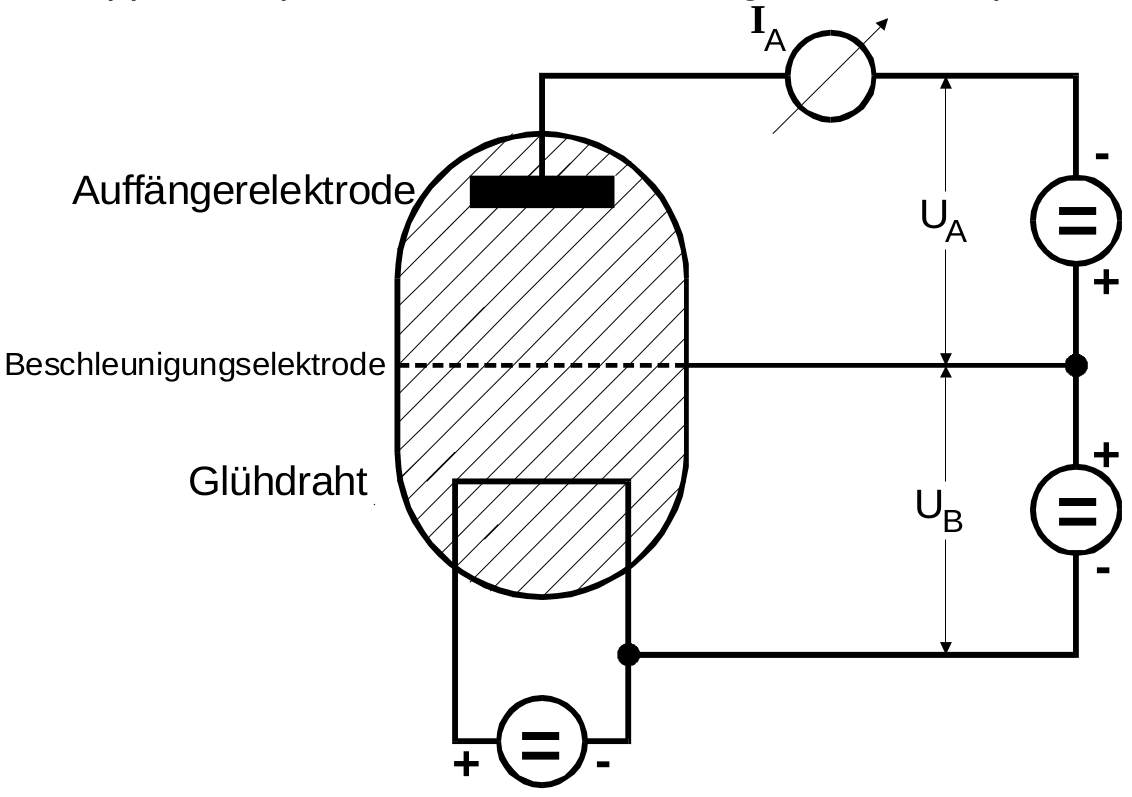
\includegraphics[width=\linewidth-170pt,height=\textheight-170pt,keepaspectratio]{content/franktheorie.png}
 \label{fig:franktheorie}
\end{figure}

Der theoretische Aufbau des Frank-Hertz Versuches folgt nach Abb.
\ref{fig:franktheorie} . Den Kern bildet eine mit Quecksilberdampf versehene und ansonsten evakuierte
Röhre. Elektronen werden über eine Glühspannung aus einer Glühkathode emittiert
und mittels einer Beschleunigungsspannung $U_\text{B}$ bis zu einer in der Mitte angebrachten
Elektrode beschleunigt. Die Elektronen haben danach die Energie
\begin{equation}
  m_0 \frac{v_\text{vor}²}{2} = e_0 U_\text{B}\text{.}\label{eq:ekin}
  \end{equation}
   Anschließend werden die Elektronen mit einer Auffängerelektrode
gefangen und der daraus resultierende Strom gemessen.
Bei Variation von $U_\text{B}$ folgt nach den bohrschen Postulaten eine
 Kurve wie in Abb. \ref{fig:Graphtheorie}.
 Bis $U_\text{B}$ größer ist als $U_\text{A}$ lässt sich kein Strom messen,
 da die Elektronen das Gegenfeld nicht durchlaufen können.
 Anschließend folgt ein Anstieg der Stromstärke,  bis die kinetische Energie
 der Elektronen $\Delta E$ übersteigt. Nun treten auch unelastische
 Stößen auf und die Elektronen verlieren nach dem obigen Modell ihre kinetische Energie.
  Daher erreichen sie die Auffängeranode nicht mehr und folgt ein plötzliches
  absinken der Stromstärke auf Null. Liegen höhere
 Spannungen an, können die Elektronen wieder ausreichend beschleunigen und die Stromstärke steigt
 wieder an, solange bis sich der Vorgang wiederholt.
 Für den Spannungsabstand zwischen 2 Stromstärkenmaxima folgt:
 \begin{equation}
   U_1 = \frac{1}{e_0}\left( E_1 - E_0 \right)\label{eq:udiff}
   \end{equation}


   \begin{figure}
   	\centering
   	\caption{Der theoretische Verlauf der Frank-Hertz-Kurve.}
   	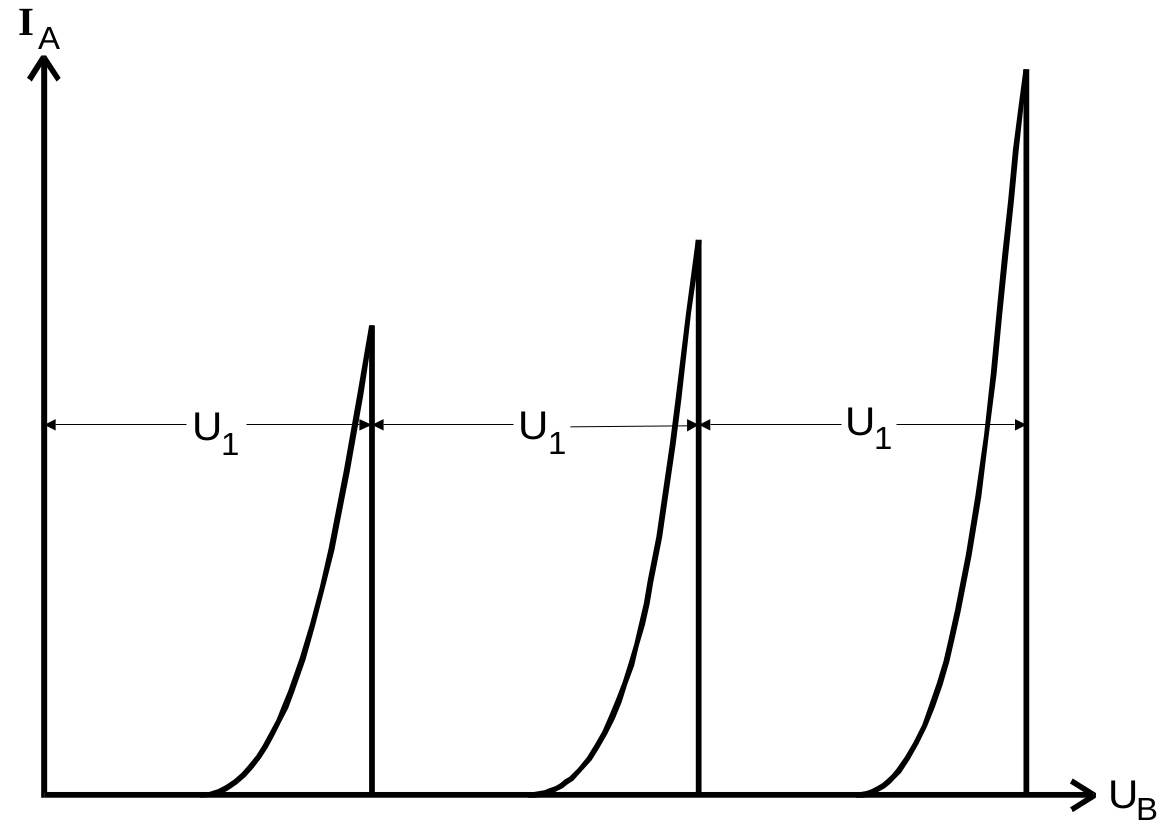
\includegraphics[width=\linewidth-170pt,height=\textheight-170pt,keepaspectratio]{content/theorie.png}
   	\label{fig:Graphtheorie}
   \end{figure}



Der in Abb. \ref{fig:Graphtheorie} dargestellte idealisierte Kurvenverlauf wird jedoch
aufgrund mehrerer Faktoren nicht erreicht.


\begin{itemize}
  \item \subsection{Die Auswirkungen des Kontaktpotentials}
  Wenn die Materialien der Glühkathode und der Beschleunigungselektrode unterschiedliche
  Austrittsarbeiten besitzen kommt es zu einer Verschiebung der effektiven $U_\text{B}$ bezüglich der
  eingestellten. Um jedoch bereits bei verhältnismäßig niedrigen Temperaturen hohe Emissionsraten
  zu erreichen, besitzt die Glühkathode ein Material mit geringer Austrittsarbeit $\Phi_\text{G}$.
  Damit es an der Beschleunigungselektrode zu keiner Elektronenauslösung wird
  für diese ein Material mit ungleich höherer Austrittsarbeit gewählt.
  %Damit es jedoch zu keiner Verfälschung der Daten durch austretende Elektronen an
  %der Beschleunigungselektrode besitzt dessen Material eine weitaus größere Austrittsarbeit
  $\Phi_\text{B}$. Es ergibt sich eine effektive Beschleunigungsspannung mit:
  \begin{equation}
    U_\text{B,eff} = U_\text{B} - K \text{ mit dem Kontaktpotential }K\text{, } K = \frac{1}{e_0}\left(\Phi_\text{B} - \Phi _\text{G} \right)\text{, }\label{eq:kontakt}
  \end{equation}
was sich in einer Verschiebung der Kurve um $K$ widerspiegelt.

\item \subsection{Das Energiespektrum der Elektronen}
Des Weiteren ist die Energie die Elektronen im Kathodenmaterial nicht einheitlich, sondern
verteilt sich gemäß der Fermi-Dirac-Verteilung. Daher treten die Elektronen mit
unterschiedlichen Anfangsgeschwindigkeiten aus und kollidieren dementsprechend
auch mit unterschiedlichen Geschwindigkeiten. %Die beobachteten unelastischen Stöße treten
%daher nicht mehr an einer fest definierten Stelle auf, sondern auf einem Bereich.
Infolgedessen fallen die Extrema geringer aus und der Graph fällt nach einem
Maximum nicht mehr unstetig auf 0, sondern nähert sich dieser asymptotisch an. Zusätzlich
ist der Einfluss der elastischen Stöße im Auffangbereich zu berücksichtigen, da die gemessenen
Ströme ausschließlich von der Geschwindigkeitskomponente in Normalenrichtung bezüglich
der Anode abhängen. %ird die Kurve durch elastische Stöße im Auffangbereich verändert,
%da weniger Elektronen das Gegenfeld durchlaufen.
Die Frank-Hertz-Kurve wird daher flacher und breiter.


\item\subsection{Die Auswirkungen des Dampfdruckes}
Damit es zu einer geeigneten Anzahl von Zusammenstößen zwischen Elektronen und Hg-Atomen
kommt, muss die mittlere freie Weglänge $\overline{w}$ der Hg-Atome klein gegenüber
der Beschleunigungsstrecke sein. Diese hängt vom vorherrschenden, temperaturabhängigen
Sättigungsdampfdruck $p_\text{sät}$ ab. Damit folgt
%mit der Dampfdruckkurve in Abb. \ref{fig:Graphdampf}
die Näherung:
\begin{equation}
  \overline{w} [cm] = \frac{0.0029}{5.5 \cdot 10⁷} \exp \left(\frac{-6876}{T}\right)\text{,}\label{eq:w}
  \end{equation}
  mit der Temperatur $T$ in Kelvin. Ist $\overline{w}$ zu groß, wächst die Wahrscheinlichkeit,
  dass Elektronen den Beschleunigungsbereich ohne Wechselwirkung durchlaufen. Ist
  $p_\text{sät}$ hingegen zu groß, treten zu viele elastische Stöße auf, welche
  die Kurve vermeidbar zerfließen lassen.
\end{itemize}

%\begin{figure}
% \centering
 %\caption{Der Verlauf der Dampdruckkurve für Hg.}
 %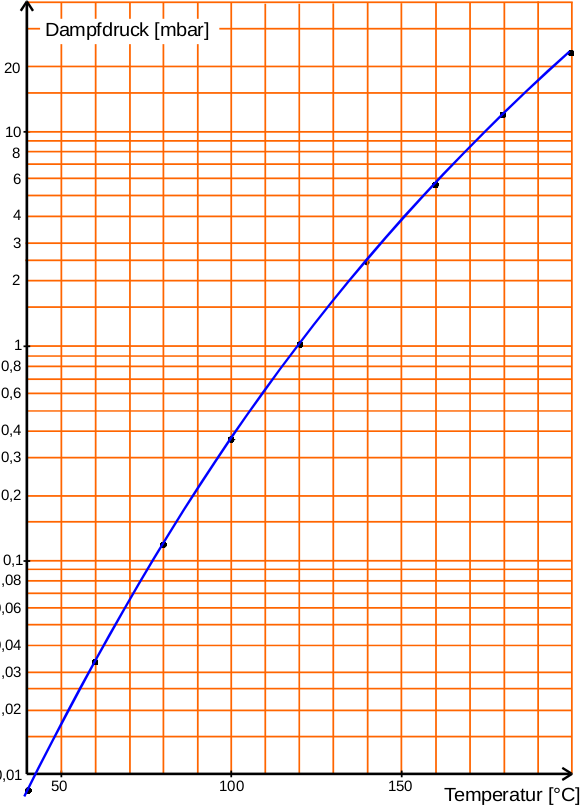
\includegraphics[width=\linewidth-170pt,height=\textheight-170pt,keepaspectratio]{content/dampf.png}
 %\label{fig:Graphdampf}
%\end{figure}
